
\chapter{Background and related work} \label{SoA}

This Chapter is meant to introduce Visual attention and how it can be modelled and evaluated.\\
Firstly we give an introduction and overview of visual attention modeling in section \ref{Introduction to Visual Attention}. Finally we will discuss Chess visual expertise in section \ref{Chess expertise and eye tracking}.
%%and finally we will introduce important layers used in our Deep learning model (section \ref{Deep learning}).

\section{ Introduction to Visual Attention} \label{Introduction to Visual Attention}

Visual attention is a biological system allowing living creature to select interesting and relevant regions from a visual scene. This gives the opportunity to higher-level cognitive functions to execute more complex task such as scene understanding or decision making while not having to focus on too much data. In cognitive neuroscience visual attention is referred as a neural system selecting information from the visual system. In his paper Posner \cite{posner1990} formulate the idea that visual attention is not the function of a singular area of the brain but rather the result of a network of different parts. He also explains that pattern recognition  is about how successions of neurons process visual stimulus to detect such information. 

Visual attention can be categorized in two ways :
\begin{itemize}
    \item Bottom-up approach : information is taken from the scene based on objects and part of the scene saliency.
    \item Top-Down : Attention is driven by task or action to accomplished based on a prior knowledge and/or the action the observer seeks to accomplish.
\end{itemize}
These two approaches are related to the two main visual attention methods. The first one being the exogenous, which is how attention component are determined by external stimulus characteristics (ie. bright object, high contrast between a hand and a background, straight lines etc..) . The second one is the endogenous, is determined by the user intentions and actions (ie. moving a chess piece, grabbing something).\\ Attention can also be described as overt or covert. Overt happens when the subject is moving his gazing point from one point to the other in the scene. Covert attention on the other hand  is also a shift in the attention/gazing point to a new location in the attention scene, but using the fovea and not a  motor action (ie. Sharp vision at a point of the scene).

Eye tracking systems detect where human eyes are fixating and they path their eyes follow. These fixations are also characterized by the time spent on different parts of the scene. These graphs of fixations and path can be used as indicators on most viewed and fixated areas on images or scenes. They are often transformed to continuous saliency maps by convoluting Gaussian functions with an higher intensity depending on the duration of fixation. Figure \ref{fig:exampleeye} shows an example of eye tracking data with in the background a chess configuration. The points are fixations with their value inside them depending on the time the user fixated this area. The line between two point is the path the eye followed between two fixations. This data was acquired through experimentation for the paper of Thomas Guntz \cite{thomasguntz}. He worked on observing and interpreting subjects in problem solving task (chess in particular) through multimodal observation (Eye tracking, posture, emotion etc...).

\begin{figure}
    \centering
    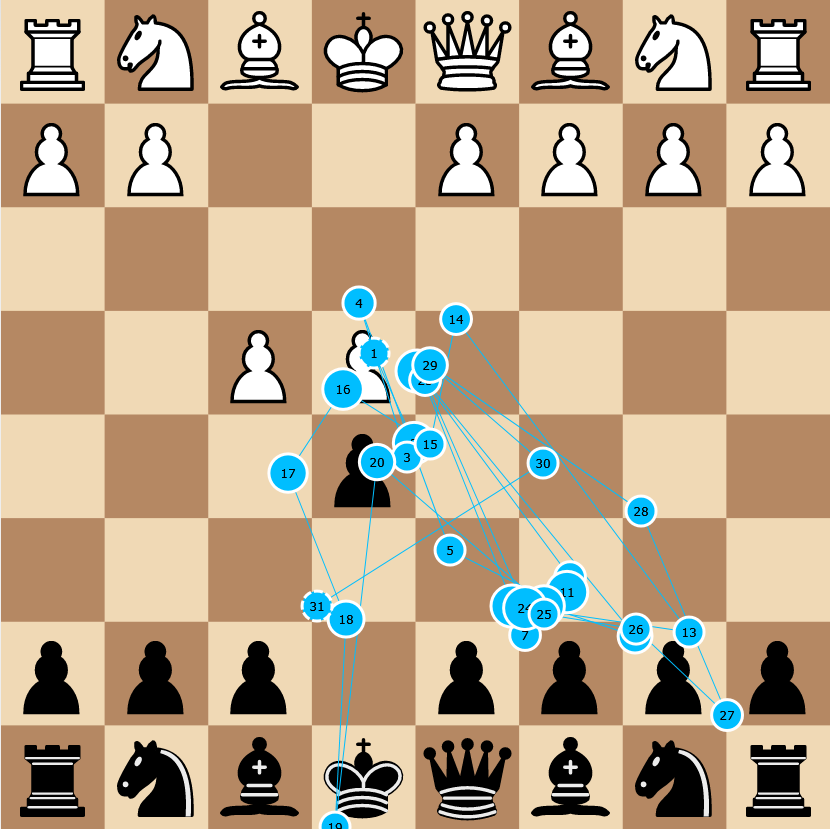
\includegraphics[scale=0.35]{./dataset/image.png}
    \caption{An example of eye tracking data for an user on a chess configuration}
    \label{fig:exampleeye}
\end{figure}

Eye tracking maps captured on human looking at a simple scene with one or few salient objects, show that they tend to notice only the main objects and ignore the background.
Chess and other board game  are particular cases for visual attention, as salient object are essentially the pieces, but their saliency is determined by their move and the current configuration of the game.



\subsection{Visual attention modeling}

Visual attention has already been subject to modeling in 1995 before the impressive development of Deep neural network , in the artificial intelligence book by Tsotsos and al \cite{tsotsos1995}.  They used a pyramidal system composed of layers and filter applied to features maps and producing saliency maps. Their work is very close to what we see nowadays with neural network and produced simple but encouraging results proving that visual attention could be modeled. Their model is based on the idea of selective tuning, features are taken from the scene and used to decide which part of it should be the center of attention, using a hierarchy of a new WAT (winner takes all) algorithm. in overall their model is strongly inspired by primate biological visual attention system, and links to biological processes such as foveating and eye movement are investigated.  \\


In their paper, Borji and Itti \cite{Borji} offer a review of techniques used in Visual attention modeling until 2013. Giving a clear overview of  different model categories such as Bayesian models, cognitive models, graphical models or spectral analysis models. Metrics are also discussed and giving a comparison between performances and approaches, they forecast what the future of visual attention modeling could be.
Circa 2012, the Deep learning field\cite{krizhevsky2012imagenet,szegedy2015going,DBLP:journals/corr/MnihKSGAWR13,jia2014caffe,5537907,deng2009imagenet,srivastava2014dropout} became the center of attention on the visual attention scene, mainly because it is a very good way to extract features automatically and use them in a bottom-up approach.
In their paper Ba and al. \cite{BaMK14}, proposed a Recurrent network model, based on visual attention to improve state of the art performances in multiple number recognition and localization. This work shows the importance of having a focused attention when comes the need to recognize an object or to locate it. However these networks learned attention, was quite different from the human one and as we are trying to model the human attention it was impossible to use the one of those network.
Xu and al. \cite{xu2015show}, worked on using salient part of the images to help a network focus its attention and generate description of images. They proposed a model capable of switching its attention between salient areas and background to offer a description of the image such as "The giraff is standing in the forest", putting in relation objects and their environment.

Visual question answering is very close to visual attention problem as for this task the network focus its attention over a region in a image to answer a question, the same way chess players would do. This is closer to the top-down approach, as the network is given an action to execute based on what he perceive. If we take apart the textual part of the problem, we end up with a "where to look at" and "what is the network looking at" problem. This is what Shih and al. \cite{DBLP:journals/corr/ShihSH15} try to tackle in their paper, where they try to find a way to express the relevancy of a region considering a question.
But most of the time as in the paper from Yang and al. \cite{DBLP:journals/corr/YangHGDS15}, attention is not really the center of preoccupation.\\

In this section we will see several ways to model visual attention before describing other methods based on deep learning (section \ref{subsub:deeplearning}).
\subsubsection{Baseline models}

Before the usage of modern deep learning techniques, a lot of model were proposed showcasing good results and interesting information about human visual attention. Some of them are presented here to give a brief idea about how we came to deep learning.\\


\textbf{Judd Model:  }In their model Judd and al. \cite{judd} worked on predicting human fixations on images. Their work has been focused on gathering data and user eye tracking fixations maps and analyzing the created dataset. Their model is composed of several SVM \cite{Cortes1995} (machine learning classification algorithm), trained on various features group (faces, colors etc..) and combined together in the end to predict fixations. Their work is remarkable for the dataset provided for future research as it was the first dataset with held-out human eye movements and is now often used as a benchmark dataset. It is composed of 300 natural indoor and outdoors scenes with 39 observers.\\


\textbf{Saliency from overt and covert mechanisms:  }In their paper, Itti and Koch \cite{ITTI20001489} proposed a model capable of attend salient locations based on different modalities such as intensity, color, or orientation. By applying filters at various scale they extract feature maps, normalized and centered and then combined to form the final saliency map. Their approach is limited to bottom-up approach but raised some good performances and helped to address how much human we carry information via saliency maps and how it can be tested.\\

\textbf{Task specific Visual Scanpath:  }Mathe and Sminchisescu \cite{NIPS2013_5196}, proposed an important dataset in visual an task driven attention, with over 1 Million fixations in 9157 images. They also developed a Markov model capable of discovering Areas of Interest (AoI), determine from eye tracking data their number, their spatial support, locations, and transition between them. They finally proposed eye movement prediction models based on reinforcement learning and advanced computer vision operators, to learn task specific visual search patterns. \\

\textbf{Bruce Model:  }The model proposed by Bruce and Tsotsos \cite{doi:10.1167/9.3.5}, is based on feature extraction (from vision operators and principal component analysis), and density estimation. Results obtained were showing great efficacy in fixation prediction as compared to other models at that time.

\subsubsection{Deep learning approaches} \label{subsub:deeplearning}
As seen previously, non deep learning models were based on known features such as colors, orientations, gradient, intensity etc.. Deep learning is based on automatic extraction of features from data and then classification, segmentation or other operations. We are going to see few deep learning approaches here, to illustrate different way  how saliency map for visual attention prediction, can be produced.\\

\textbf{SALICON:  }In 2015, SALICON \cite{7410395} was a paper proposing a novel technique based on Deep Neural Networks and object recognition for predicting visual attention. They based their work on the gap of predicting eye fixation with a big semantic content, and previous method proposed, thanks to the high-level encoding in Deep neural networks. They worked on fine-tuning the network with objective functions based on saliency evaluation and by integrating information from the image at different scales. Even today this model is still ranked with the top scores on most of the metrics (described in section \ref{seq:metrics}. 0.87 with AUC-Judd,0.74 linear correlation etc..).

\textbf{Deep fix :  }Deepfix \cite{DBLP:journals/corr/KruthiventiAB15} is a fully convolutional model learning features at different scale, but thanks to a "Location biased convolution layer" it allows to model location dependent patterns. This location problem is addressed by concatenating Gaussian blobs to the input of the convolution layer. They also introduced inception layers to extract complex semantic a different scales level and  to capture global context with large receptive fields.\\

\textbf{Deep Gaze 2:  }DeepGaze 2 \cite{Kummerer_2017_ICCV} is a network meant to be simpler than previous approaches with a pre-trained first part based on VGG19\cite{DBLP:journals/corr/SimonyanZ14a} followed by a readout network. The readout network is a succession of 1*1 convolutions producing a saliency map which is then blurred and transformed into a probability distribution by a softmax function. It uses log likelihood as a loss function to optimize. It produces to this day the best result for the AUC-Judd metric (0.88).\\

\textbf{Salgan: }Finally SalGAN \cite{DBLP:journals/corr/PanCMOTSN17} offers a complete different approach from what we have seen before. This network is a Generative adversarial Networks (GAN \cite{2014arXiv1406.2661G}) composed of a generator and a discriminator. The latter is composed of convolutions (here trained from scratch), follows by  pooling functions  and a fully connected last part. The Generator is an autoencoder , with a first part composed of a VGG network followed by upsampling functions and  a sigmoid. A binary cross entropy loss is computed between the saliency map generated by the generator and the ground truth. Both ground truth and predicted saliency map are given as input to the discriminator which is then  doing predicting and  training using adversarial loss.
This paper is also interesting as it gives a comparative analysis between the Binary cross entropy loss and the Mean square error loss, two loss which can be used with autoencoder, for saliency map generation.

\textbf{Deep visual attention:  } Deep visual attention \cite{DBLP:journals/corr/WangS17b} is a recent paper aiming to leverage multi-scale features for attention prediction model. They use and autoencoder but the decoder is separated into several part, each of them predicting saliency 
for the output of different layers of the encoder. The prediction of the encoders are fused using a last convolutional layer. Their work not only figure in the best performances for attention prediction in view-free scenes (0.85 for AUC-Judd and 0.688 for linear correlation, on the MIT300 dataset \cite{Judd_2012}), but also propose a way to take in consideration multi-scale and spatial relationship in them.


From what we have seen, there exists many ways of approaching visual attention prediction using deep learning. Because of the relations between pieces in chess and the importance of using various scales of features to recognize pieces and moves, we choose to base our model on the Deep visual attention model \cite{DBLP:journals/corr/WangS17b}, but adding some changes as we will see in section \ref{section:model}.

\subsection{Measuring Visual attention}\label{seq:metrics}
To measure quality of saliency map, we consider them as probability distribution. Several metrics can be used and some of them are explained in this section of the report. More about those metrics and some others can be found it Bylinskii and al. \cite{metricsreview}, where they explain the interpretation that can be done depending on the results we can get. They also show how changing the distribution create variation on the results.THree years before Le Meur and Baccinon \cite{LeMeur2013}, proposed a survey for various models for visual attention where they emphasize the use of some methods to benchmark computational models of visual attention.
In this section we will present some of the main metrics used in visual attention prediction.

\subsubsection{Normalized Scanpath Saliency}
Normalized Scanpath Saliency was introduced in Peters and al. paper \cite{Peters2005ComponentsOB}, as a correspondence measure between a normalized saliency map a ground truth at fixations. It is sensible to false positives, relative differences  in  saliency  across  the  image,  and  general   monotonic  transformations. But because of the mean saliency value being subtracted, it is robust to linear transformations. The formula to compute this metric is given in equation \ref{eq:NSS}, Q being our binary ground truth and P the saliency map produced by our model. 

\begin{equation}  
\begin{aligned}
    NSS(P,Q) = \frac{1}{N} \sum\limits_{i=0}^n \bar{P_i} * Q_i\\
    \textrm{where} \quad  \bar{P}= \frac{P - \mu(P)}{\sigma(P)} \quad \textrm{and} \quad  N =  \sum\limits_{i=0}^n Q_i
\end{aligned}
\label{eq:NSS}
\end{equation}
With a value above 0, this metric expresses a correspondence above chance between the two saliency, and below 0 an anti-correspondence.

\subsubsection{Similarity}
Similarity or also referred as histogram intersection is the sum of minimums of two normalized saliency maps. It is defined in equation \ref{eq:SIM} where P is the saliency map produced by the model, and Q the ground-truth.
\begin{equation}  
\begin{aligned}
    NSS(P,Q) = \sum\limits_{i=0}^n min(P_i, Q_i)\\
    \textrm{where} \quad \sum\limits_{i=0}^n P = \sum\limits_{i=0}^n Q = 1
\end{aligned}
\label{eq:SIM}
\end{equation}
At 0 the similarity show that their is no overlap and a sim of one indicates that the saliency maps are the same.

\subsubsection{Linear Correlation Coefficient}
Linear correlation is a statistical method to determine how much two probability distributions are related one to the other. It is asserted in equation \ref{eq:CC}, where $cov$ is the covariance between the two distributions, and $\sigma$ their standard deviation.
\begin{equation}  
\begin{aligned}
    CC(P,Q) = \frac{cov(P,Q)}{\sigma(P)*\sigma(Q)} 
\end{aligned}
\label{eq:CC}
\end{equation}
The value given by the linear correlation has a range between -1 and +1, the closer to +1 or -1 it gets, the more related the two distributions are. Because of its symmetric computation, linear correlation don't do the difference between false positive and false negative. 

\subsubsection{Earth mover's distance}
Metrics previously mentioned are mostly about the dissimilarity between two distribution at each pixels but don't take into account the spatial distance between them. Earth mover's distance (EMD), is about computing the minimum cost to change one distribution into the other. Very robust metric for image matching, the total cost is the amount of density moved time the distance between it source and destination. The equation \ref{eq:EMD} shows how to compute this distance for two distributions.

\begin{equation}  
\begin{aligned}
    EMD(P,Q) = min_{f_i} \sum\limits_{i,j} f_{ij} d_{ij} + \vert\sum\limits_{i} P_i \sum\limits_{j} Q_j \vert  max(d_{ij}) \\
    \textrm{Contraints : }\\
    f_{ij}  \geqslant 0 \quad \textrm{;} \quad  \sum\limits_{j} f_{ij} \leqslant P_i \quad \textrm{;} \quad \sum\limits_{j} f_{ij} \leqslant Q_j\\  \sum\limits_{i,j} f_{ij} = min(\sum\limits_{i} P_i \sum\limits_{j} Q_j)
\end{aligned}
\label{eq:EMD}
\end{equation}
In equation \ref{eq:EMD}, $f_{ij}$ is the amount of density moved from pixel i to j, and $d_{ij}$ the distance between i and j. P and Q are the two distributions. The first constraint allows to move density to go from P to Q and not the other way. The  next two constraint  express the fact that we cannot move density more than we can get in pixel i and that we cannot put more at j than there are in the goal distribution Q. The last constraint just tells that we cannot move more density than there is either in P or Q. Basically this metric is solving an optimization problem on the map P and is computationally expensive especially for large distributions. A large EMD shows a larger difference between the two distributions. At 0, the two distributions are the same. 

\subsubsection{Area under the curb (AUC)}
The main goal in visual attention modeling is to predict if a pixel is going to be fixated or not, which is basically a binary classification (fixated or not). The ROC (Receiver Operating Characteristic) is in signal detection theory a measure of the trade off between true an false positives while making some variations in threshold (examples of threshold variations can be seen in figure \ref{fig:threshsal}). The article from Tom Fawcett \cite{FAWCETT2006861} offers a great introduction to this metric and is a good guide about how to use it and understand it. 
For saliency evaluation, we consider the saliency map as a binary classifier, changing the threshold and measuring the true and false positive rate. The AUC metric is then the area under the ROC curve, and even if different implementations exist, the difference between them is how the true and false positive values are computed.\\


\begin{figure}[ht!]
    \centering
    \begin{tabular}{@{}c@{\hspace{0.1cm}}c@{\hspace{0.1cm}}c@{\hspace{0.1cm}}}
        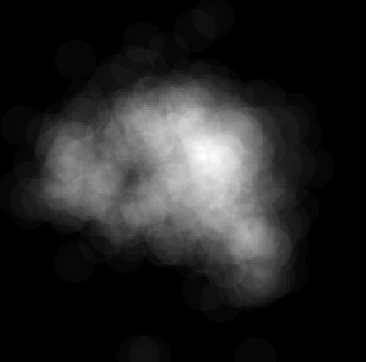
\includegraphics[width=0.25\linewidth]{./pics/saliency_map.png}& 
        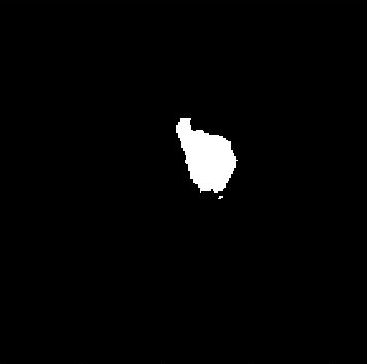
\includegraphics[width=0.25\linewidth]{./pics/2per.png}&
        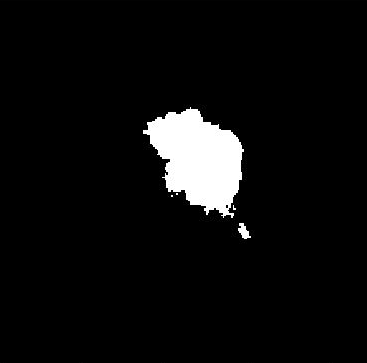
\includegraphics[width=0.25\linewidth]{./pics/5per.png}\\
        {\small  Saliency map} & {\small 2\% threshold} & {\small 5\% threshold}\\
     \end{tabular}
    \begin{tabular}{@{}c@{\hspace{0.1cm}}c@{}}
        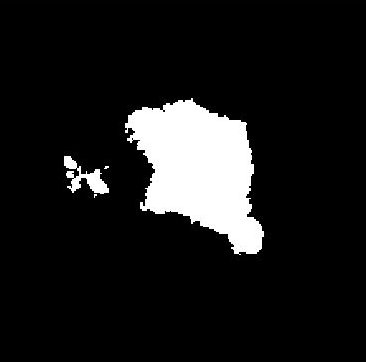
\includegraphics[width=0.25\linewidth]{./pics/10per.png}& 
        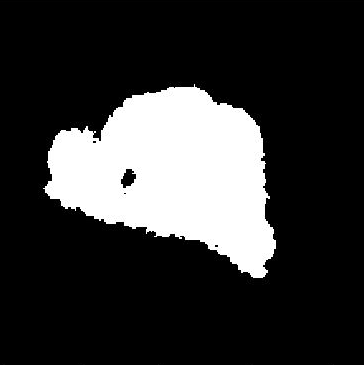
\includegraphics[width=0.25\linewidth]{./pics/20per.png}\\
        {\small  10\% threshold} & {\small 20\% threshold}\\
    \end{tabular}
    \caption{A saliency map and its binary transformation following different thresholds}
    \label{fig:threshsal}
\end{figure}

\textbf{AUC-Judd}\\

AUC-Judd gets its name from the work of Judd and al. \cite{judd,Judd_2012,metricsreview}. For a given threshold the true positive rate is the ratio of true positives by the total numbers of fixations, true positives being values above the threshold at fixated pixels on the ground truth. False positives rate is also the false positives over the number of saliency map pixels at the given threshold. False positives are saliency values above the threshold at unfixated pixels in the ground-truth. \\

\textbf{AUC-borji}\\

From the Borji's work \cite{6751224} we get an other variant of AUC called AUC-Borji. The true positive rate is the same as AUC-Judd, but the false positive rate is the ratio of saliency map values above threshold sampled at random pixels (as many as fixations, sampled uniformly above the whole image), over the number of saliency map pixels at a given threshold. 


The last saliency maps AUC implementation is shuffled AUC \cite{sAUC}. It is meant to penalize models with a center bias.



\section{Chess expertise and eye tracking}\label{Chess expertise and eye tracking}


\textbf{Do an Introduction}


\subsection{Reingold and visual expertise}
Eyal Reingold is a Doctor in psychology who worked on perception and how chess players, depending on their expertise level, were looking at a chess configuration. In a paper from 2001 \cite{Charness2001},him and Charness discovered that experts compare to intermediate players, produce more fixations on empty squares. Also when fixating pieces, the number of fixations on relevant pieces was way greater. It was argued that experts were encoding configurations rather than pieces and produced patterns of saccading (quick movement of eyes between two or more phases of fixation).\\
In an other paper \cite{Perceptioninchess}, Charness and Reingold, demonstrated larger visual spans for expert players while processing structured chess positions. They also show that those experts player rather than fixating large number of pieces, would make fewer fixations and rather look at relation between pieces than on pieces. Finally an important idea that we can take from this work is that chess piece saliency influences the saccadic endpoints for experts making their encoding part faster than  intermediate players.\\
In a more recent paper  \cite{doi:10.1167/17.3.4} he presented the fact that chess expertise is mainly related to the detection of complex patterns and configurations. When improving our level, we become capable of detecting patterns in the pieces positions. This is why expert don't need to fixate pieces, and instead detect an interesting pattern by looking at its center.

\subsection{Using players level to aggregate their eye tracking data}
From the previous sub-section information we have an idea of how depending on the chess configuration and the player's level, the saliency map would look like. Taking only expert players and aggregating their data would give us very salient areas in the center of configurations and more focused on empty cells than on pieces as the Figure \ref{fig:fixationsempty} shows.\\
For intermediate players we should have a more spread salient area, including relevant pieces to the configuration. Adding less good players data, the salient area would concentrate toward pieces and would be more spread across the board, looking for "major" pieces such as queens,rooks,bishops...\\

\begin{figure}
    \centering
    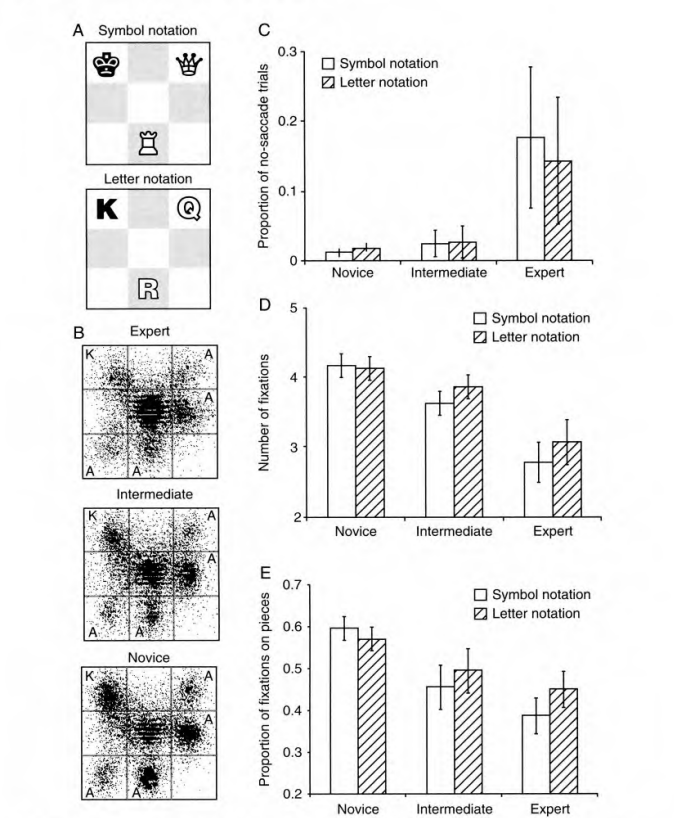
\includegraphics[scale=0.35]{./results/reingold_emptypieces.png}
    \caption{A figure on fixations of chess player from \cite{doi:10.1167/17.3.4}. In the left column we have the in A the notation of pieces and B the Scattergrams of gaze positions, for a check detection task (letter A represents an attacked piece position and K the king). In the right column we have the proportion of no-saccade trial (not moving the eyes from the center position and trying to solve the task), the number of fixations and the number of fixations on pieces for each level of players.}
    \label{fig:fixationsempty}
\end{figure}

Datasets in visual attention aggregate visual saliency maps of all users on images just by summing them up. This strategy, works pretty well since for images such as portraits or landscape, humans tend to look at them the same way and focus on quite similar points. As an example, a human face would be more salient around the eyes and mouth as this characterize us and make us see a face.
This way of aggregating data would work with chess, if our users would be only experts or intermediates. Otherwise just summing saliency maps would in the end create wide salient areas, not really characterizing human visual attention on the chessboard. We use instead an averaging method discussed later in the report ( section \ref{section:data}), taking at each pixels the average of values across the user.



    
    